\documentclass[useAMS, usenatbib]{mnras}
\pdfsuppresswarningpagegroup=1
%
\usepackage[spanish,es-minimal,english]{babel}
\usepackage[utf8]{inputenc}
\usepackage{graphicx}

\usepackage{xcolor}
\usepackage{hyperref}
\usepackage{siunitx}
\usepackage{newtxtext}
\usepackage[stix2,smallerops]{newtxmath}
\usepackage{booktabs}
\hypersetup{colorlinks=True, linkcolor=blue!50!black, citecolor=black,
  urlcolor=blue!50!black}
\usepackage{etoolbox}
\robustify\bfseries
\robustify\itshape

\usepackage[shortlabels]{enumitem}

\bibliographystyle{mnras}

\sisetup{
  % explicit "+" is useful for velocities
  retain-explicit-plus = true,
  % prefer 10^6 over 1 x 10^6
  retain-unity-mantissa = false,
  % Use x +/- e instead of x(e)  
  separate-uncertainty = true,
  % Make sure to pick up bold font when used in section heading for instance
  detect-weight = true,
}

%% 
%% Will macros
%%
% A better \ion command that works in more circumstances
\newcommand\ION[2]{#1\,\scalebox{0.9}[0.8]{\uppercase{#2}}}
\newcounter{ionstage}
\renewcommand{\ion}[2]{\setcounter{ionstage}{#2}% 
  \ensuremath{\mathrm{#1\,\scriptstyle\Roman{ionstage}}}}
\newcommand\hii{\ion{H}{2}}
\newcommand\nii{[\ion{N}{2}]}
\newcommand\oiii{[\ion{O}{3}]}
\newcommand\oii{[\ion{O}{2}]}
\newcommand\Wav[1]{\ensuremath{\lambda #1}}

\title[HH 529 II and III in the Orion Nebula]{
  Photoionized Herbig-Haro objects in the Orion Nebula I: HH 529 II and III
}

\author[J. E. M\'endez-Delgado et al.]
{J. E. M\'endez-Delgado$^{1,2}$ \thanks{E-mail: jemd@iac.es},
  C. Esteban$^{1,2}$, J. Garc{\'{\i}}a-Rojas$^{1,2}$, W. J. Henney$^{3}$  
  \newauthor 
  and K. Z. Arellano-C\'ordova$^{1}$ and collaborators\\
\\
% List of institutions
$^{1}$Instituto de Astrof\'isica de Canarias (IAC), E-38205 La Laguna, Spain\\
$^{2}$Departamento de Astrof\'isica, Universidad de La Laguna, E-38206 La Laguna, Spain\\
$^{3}$Instituto de Radioastronom\'ia y Astrof\'isica, Universidad Nacional Aut\'onoma de M\'exico, Apartado Postal 3-72, 58090 Morelia, Michoac\'an, M\'exico}


\begin{document}

\begin{table}
  % Fake the labels for some Tables
  \setcounter{table}{3}\caption{}\label{tab:pc}
  \setcounter{table}{12}\caption{}\label{tab:total_abundances_rls}
\end{table}

\addtocounter{section}{11}
\section{Physical aspects of the high velocity components}
\label{sec:phys-aspects-high}


\newcommand\Mach{\ensuremath{\mathcal{M}}}
\newcommand\shock{\ensuremath{_{\mathrm{sh}}}}
\newcommand\sound{\ensuremath{c_{\mathrm{s}}}}
\newcommand\ws{\ensuremath{_{\mathrm{WS}}}}
\newcommand\jet{\ensuremath{_{\mathrm{jet}}}}
\newcommand\env{\ensuremath{_{\mathrm{env}}}}
Since the material in the HH outflows is moving highly supersonically
with respect to the ionized sound speed in the nebula,
it will give rise to shocks where the flow and nebula interact
\citep{Hartigan:1987a}.
Further internal shocks may form inside the outflow
if its velocity varies with time \citep{Raga:1990a}.
It is important to investigate the degree to which direct excitation by the shocks
might be affecting our emission line analysis.

In this section,
we first calculate the heating and compression expected behind a shock wave.
Second, we estimate the range of likely shock velocities expected to be
found in the HH~529 knots.
Third, we use results of non-equilibrium Cloudy simulations to predict the relative contributions of the post-shock cooling zone and the
equilibrium photoionized shell to the emission line spectrum of the knots.

\subsection{Shock compression and heating}
\label{sec:shock-compr-heat}

A non-magnetised hydrodynamic shock is characterized by its Mach number \(\Mach = V\shock / \sound\),
where \(V\shock\) is the shock velocity and \(\sound\) is the pre-shock adiabatic sound speed.
On passing through the shock, the gas is heated 
\citep{ZelDovich:1967a} to a temperature \(T_1\),
which is higher than the equilibrium photoionized temperature, \(T_0\):
\begin{equation}
  \label{eq:T1-T0}
  \frac{T_1}{T_0} = \frac{1}{16} \bigl( 5 \Mach^2 - 1 \bigr)
  \bigl( 1 + 3\Mach^{-2} \bigr),
\end{equation}
while at the same time it is compressed by a factor
\begin{equation}
  \label{eq:rho1-rho0}
  \frac{\rho_1}{\rho_0} = \frac{4 \Mach^2}{\Mach^2 + 3} .
\end{equation}
In both cases, a ratio of specific heats \(\gamma = 5/3\) is assumed,
as is appropriate for ionized and atomic gas. 
The post-shock gas then cools in a radiative relaxation layer
until it returns to the equilibrium temperature \(T_2 \approx T_0\),
reaching a final density compression factor of 
\begin{equation}
  \label{eq:rho2-rho0}
  \frac{\rho_2}{\rho_0} = \frac53 \Mach^2 .
\end{equation}

The adiabatic sound speed in the equilibrium ionized gas is given by
\(\sound = (\gamma k T / \mu m_{\mathrm{H}})^{1/2}\),
where \(k\) is the Boltzmann constant, \(T\) is the temperature,
\(m_{\mathrm{H}}\) is the hydrogen mass
and \(\mu\) is the mean atomic mass per particle.
Assuming that all He is singly ionized with
\(y = \mathrm{He/H} = 0.087\) (Table~\ref{tab:total_abundances_rls}) yields
\(\bar{m} \approx (1 + 4 y) / (2 + 2 y) \approx 0.62\),
which combined with \(T = \SI{8480}{K}\) (Table~\ref{tab:pc})
implies an adiabatic sound speed of \(\approx\SI{13.7}{km.s^{-1}}\). 

The case of a magnetized shock is considerably more complicated \citep{Bazer:1959a},
but the principle effect is that the component of the magnetic field, \(B\), parallel to the shock front provides extra pressure support (magnetic cushioning) in the post-shock gas \citep{Hartigan:1994a}.
An approximate way to account for this is to replace the sound speed in the above equations by the fast magnetosonic speed: \(V_{\text{fast}} = (\sound^2 + V_{\text{A}}^2)^{1/2}\), where \(V_{\text{A}} = B / (4\pi \rho)^{1/2}\)
is the Alfvén speed.
The ambient gas inside an \hii{} region is expected to have a low
Alfvén speed of \(V_{\text{A}} \approx \SI{2}{km.s^{-1}} \ll \sound\)
\citep{Arthur:2011a}
so that the magnetic cushioning will be negligible
in shocks propagating in the ambient medium.
On the other hand,
the Alfvén speed in the jet itself \citep{Hansen:2015b, Pudritz:2019a}
may be sufficiently high so as to limit the compression behind
shocks driven into the jet.

\subsection{Shock velocities in jet working surfaces}
\label{sec:shock-velocities-jet}


\begin{figure}
  \centering
  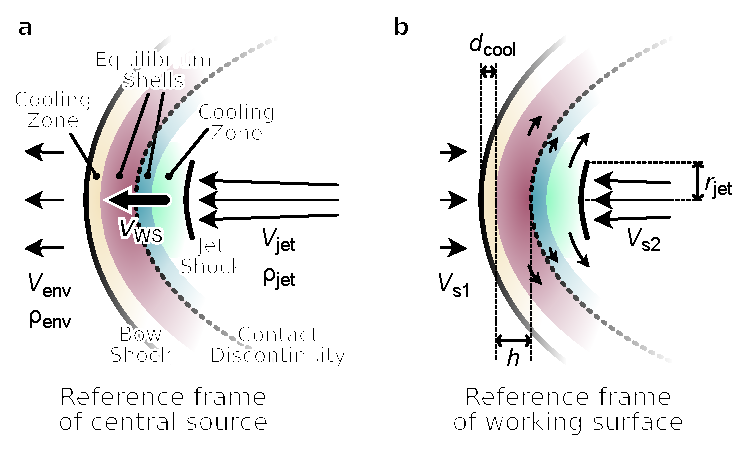
\includegraphics[width=\linewidth]{working-surface-diagram}
  \caption{
    Structure of a fully photoionized jet knot,
    modeled as a steady-state working surface,
    which forms when a jet propagates supersonically into an environment.
    (a)~Velocities in the frame of reference of the central jet source.
    (b)~Velocities in the frame of reference of the working surface.
  }
  \label{fig:working-surface}
\end{figure}

\begin{figure}
  \centering
  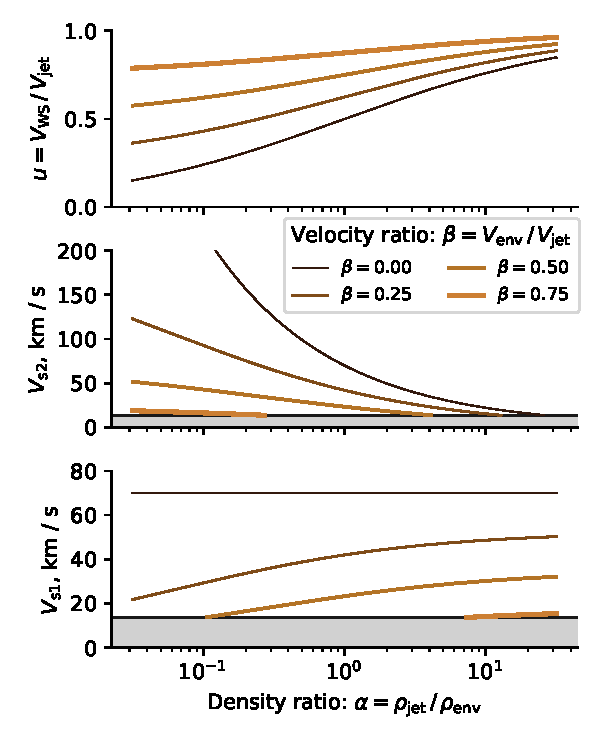
\includegraphics[width=\linewidth]{shock-velocities}
  \caption{Inner and outer shock velocities of a working surface
    as a function of the jet-to-environment ratio of density and velocity
    (\(\alpha\) and \(\beta\)).
    Upper panel shows the pattern speed of the working surface, \(V\ws\),
    in terms of the jet velocity, \(V\jet\).
    Middle panel shows the velocity of the jet shock, \(V_{\mathrm{s1}}\),
    for the case where \(V\ws = \SI{70}{km.s^{-1}}\).
    The gray shaded area indicates subsonic velocities where no shock exists. 
    Bottom panel is the same but for the bow shock \(V_{\mathrm{s2}}\).
  }
  
  \label{fig:shock-velocities}
\end{figure}

Figure~\ref{fig:working-surface} illustrates a simplistic model of the structure of a jet knot.  An outer shock (the bow shock) accelerates the environment, while an inner shock (the jet shock or Mach disk) decelerates the jet.
The region between these two shocks comprises shocked environment and jet material in approximate pressure equilibrium,
which is denoted the working surface.
The speed of the working surface with respect to the jet source, \(V\ws\),
will only be a fraction of the jet speed: \(u \equiv V\ws / V\jet\)
(see Figure~\ref{fig:working-surface}a),
depending on the velocities and densities of the jet and environment,
which we characterize by the ratios \(\alpha = \rho\jet/\rho\env\) and \(\beta = V\env/V\jet\).
For the terminal working surface with which the jet interacts directly with the nebula, one expects \(\beta \approx 0\),
whereas internal working surfaces due to jet variability may have \(\beta \sim 0.5\).
Assuming that the momentum transfer efficiency from the jet to the working surface is the same as that from the environment
and additionally that \(V\jet \gg \sound\), then ram pressure balance yields
\begin{equation}
  \label{eq:u}
  u = \frac{(1 - \beta)\alpha^{1/2} - (\alpha - \beta)}{1 - \alpha} , 
\end{equation}
which is shown in the upper panel of Figure~\ref{fig:shock-velocities}.
The shock velocities are then given by 
\(V_{\text{s1}}/V\jet =  (u - \beta)/u \) for the bow shock,
and \(V_{\text{s2}}/V\jet = (1 - u)/u \) for the Mach disk.
These are shown in the lower two panels of Figure~\ref{fig:shock-velocities}
for the case where \(V\jet = \SI{70}{km.s^{-1}}\).

In reality, the knot structure may be more complicated
with internal clumps \citep{Hansen:2017a, Yirak:2009a, Yirak:2012a}
and the possibility of double working surfaces \citep{Raga:2017b}.  



\subsection{Shock emission versus shell emission}
\label{sec:shock-emiss-vers}



\bibliography{will-529-shock-refs}

\end{document}

%%% Local Variables:
%%% mode: latex
%%% TeX-master: t
%%% End:
